The HLT shares the same code used for offline data processing, thus the processing pipeline is more or less the same. The fundamental difference is that the output is used to perform event classification instead of data analysis. 
\begin{figure}[ht]
  \centering
  \caption{HLT processing pipeline}
  \label{img:hlt}
  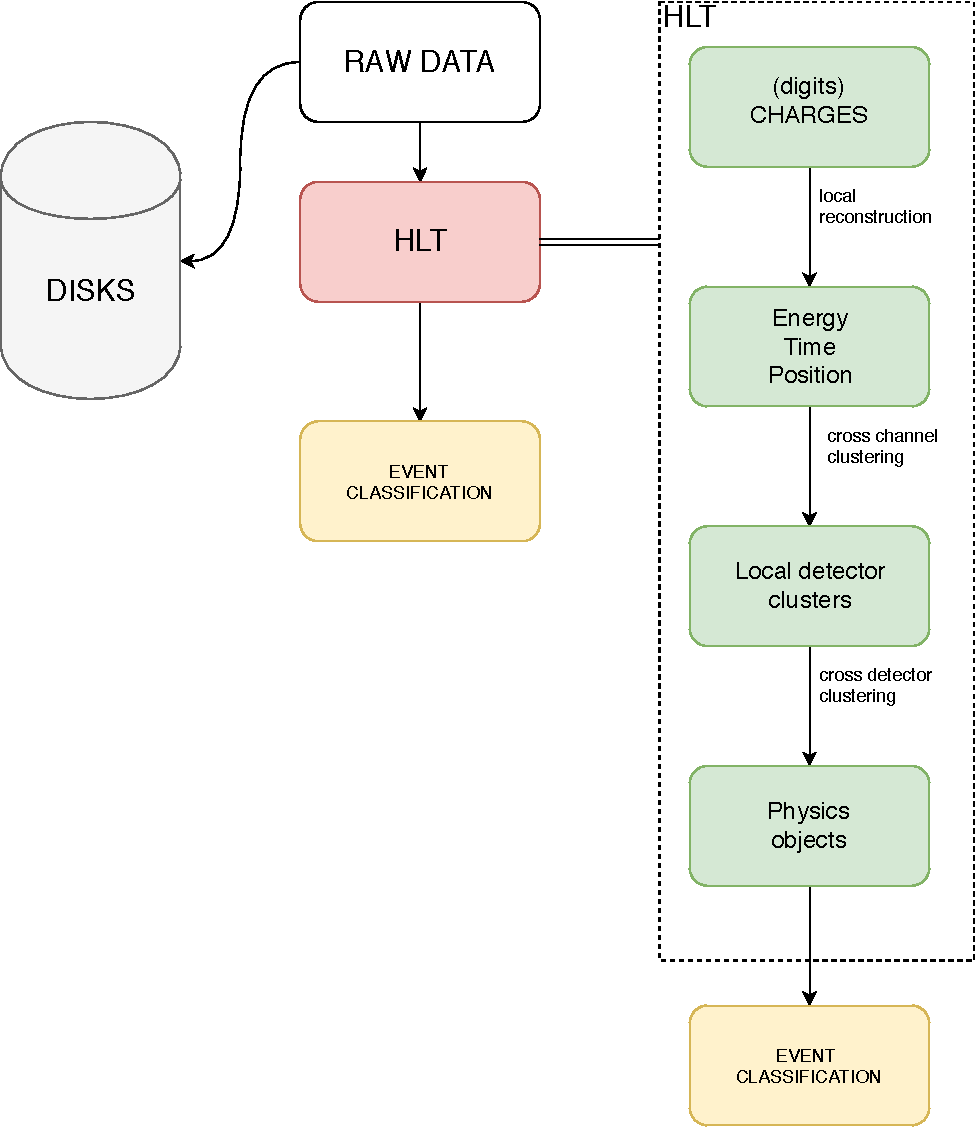
\includegraphics[width=.70\textwidth]{img/hlt}
\end{figure}
The table \ref{table:timeshare} shows how much time is spent in every single step of the reconstruction process. Most of it is spent into tracking but after it, the second more time consuming step is HCAL+ECAL local reconstruction that takes $113 ms$ corresponding to $24\%$ of the total time.
\begin{figure}[ht]
  % \centering
  \caption{Data processing time share}
  \label{img:hlt}
  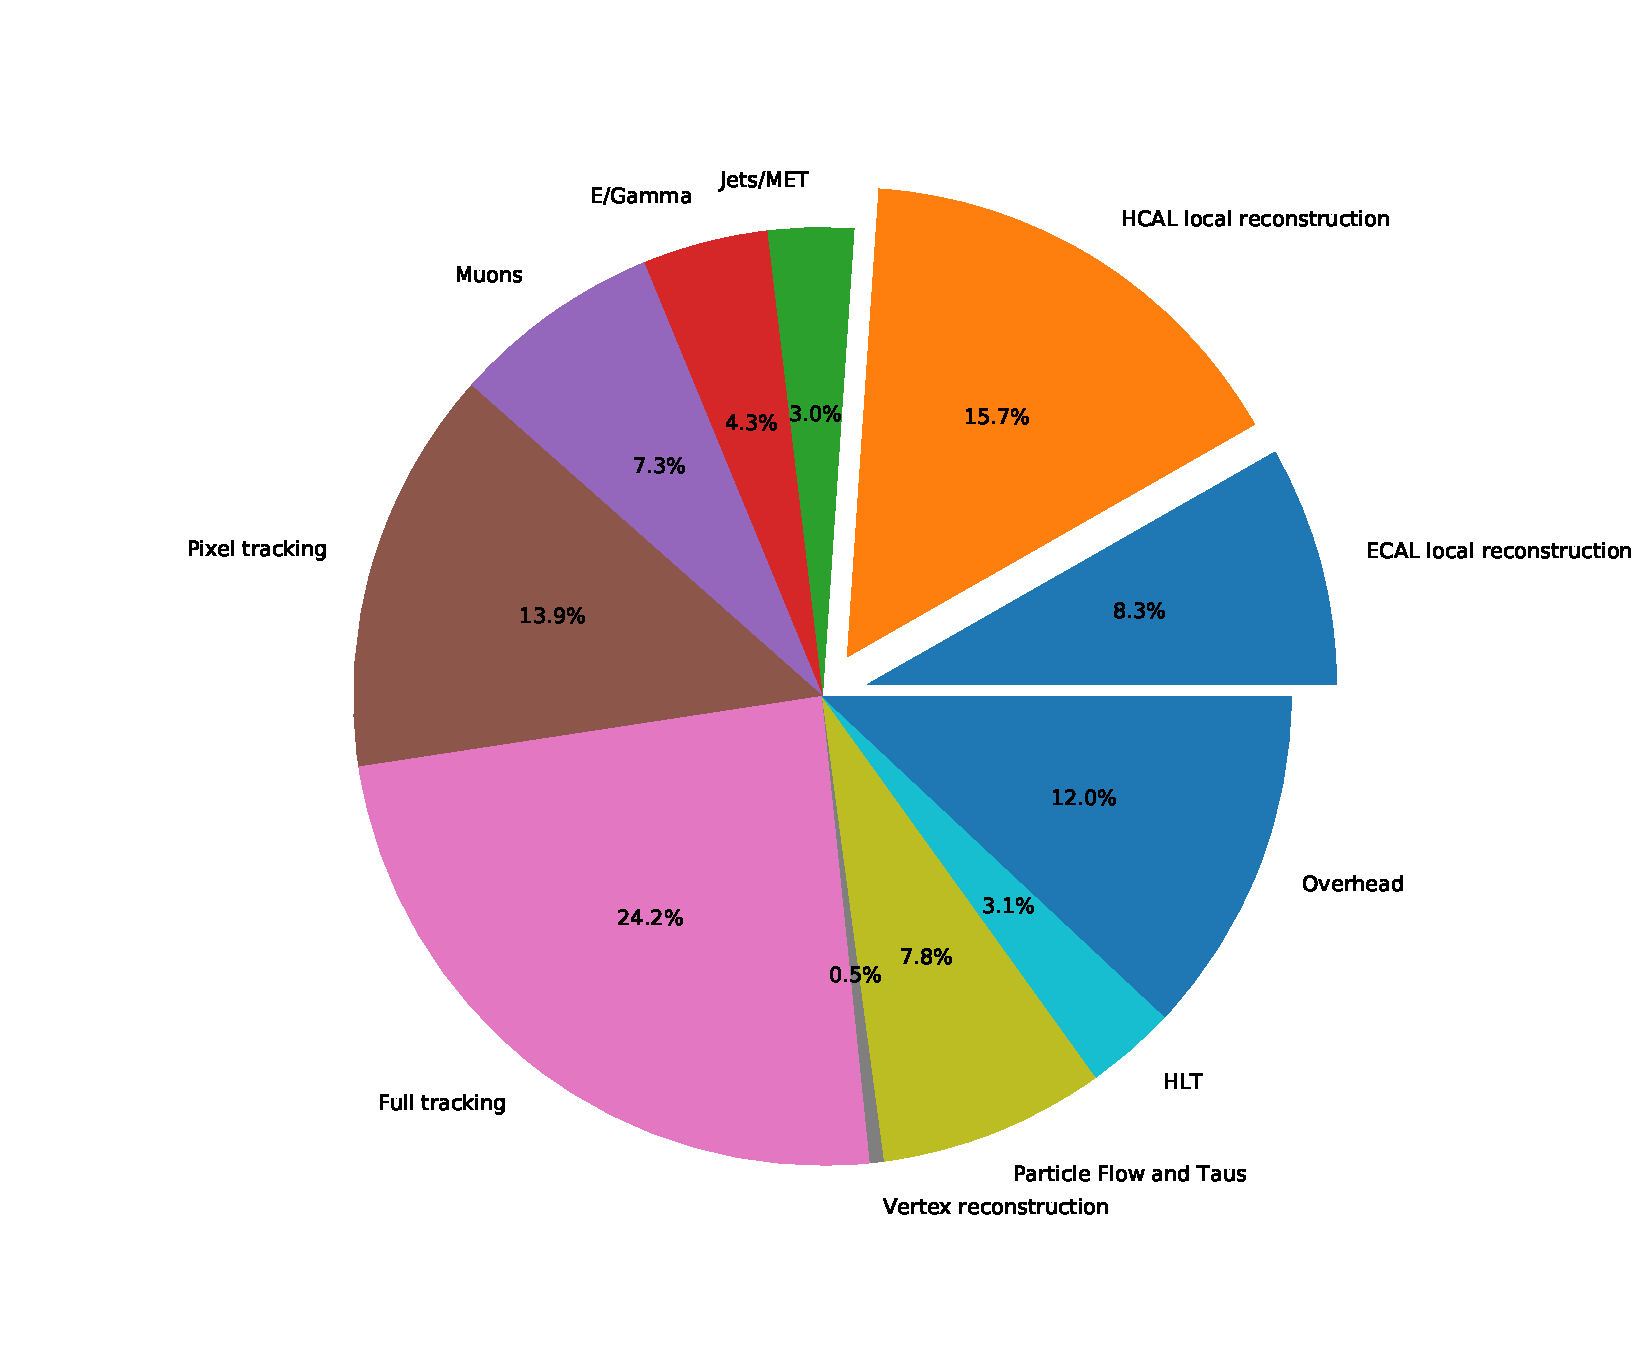
\includegraphics[width=\textwidth]{img/timeshare}
\end{figure}
\begin{table}[ht]
  \caption{Time spent into the various HLT reconstruction steps}
  \label{table:timeshare}
  \begin{tabular}{lll}
    \hline
    Step                      & Real-Time      & Percentage \\ \hline
    ECAL local reconstruction & 38.9 ms        & 8.25\%     \\
    HCAL local reconstruction & 73.9 ms        & 15.67\%    \\
    Jets/MET                  & 14 ms          & 2.97\%     \\
    E/Gamma                   & 20.4 ms        & 4.33\%     \\
    Muons                     & 34.2 ms        & 7.25\%     \\
    Pixel tracking            & 65.7 ms        & 13.93\%    \\
    Full tracking             & 114.2 ms       & 24.22\%    \\
    Vertex reconstruction     & 2.3 ms         & 0.49\%     \\
    Particle Flow and Taus    & 36.8 ms        & 7.8\%      \\
    HLT                       & 14.7 ms        & 3.12\%     \\
    Overhead                  & 56.4 ms        & 11.96\%    \\
    Total                     & 471.5 ms       & 100\%      \\ \hline
  \end{tabular}
\end{table}
Given the time needed to perform this reconstruction even achieving a speedup of two would reduce the total processing time by more than $10\%$. This is the focus of this project: try to reduce it as much as possible by both optimizing it for CPU and exploiting GPU resources.
\section{Problem statement}
For each channel \{given $n$ charge readouts $\rightarrow$ reconstruct the energy\}. \\
\begin{equation}\label{eq:chisq}
  \begin{split}
    & \min(\chi^2)=\arg min_x(\norm{Px - b}^2) \\
    & \forall i: x_i \geq 0\\
    \text{where:}&  \\
    & x = \text{energy vector} \\
    & P:ENERGY \rightarrow CHARGE =\text{feature matrix} \\
    & b = \text{charge vector}\\
    & n = 10 \text{ (in this particular case)}
  \end{split}
\end{equation}
Which is a standard min$\chi^2$ problem with additional positivity constraints. This constraint is present because physically speaking negative energy does not make sense. \\
As shown in \cite{amplituamplitude_reconde_recon} the statement above is incomplete. A perfect mapping from charges to energy does not exist because signal from the shower does not dissipate within one time slice ($25ns$). Adding the correlation term this problem becomes:
\begin{equation}\label{eq:constrained_chi_sq}
  \begin{split}
      &\arg min_x(\norm{(Px - b)^T\Sigma(x)^{-1}(Px - b)}^2) \\
      & \forall x: x \geq 0\\
  \end{split}
\end{equation}
It is worth pointing out that $\Sigma$ depends on x, meaning also $\Sigma$ is unknown. \\
To compute $\Sigma$ an iterative procedure is used:
\begin{enumerate}
  \item Compute $\Sigma$.
  \item Minimize $\chi^2$.
  \item If not convergence goto 1.
\end{enumerate}
More precisely $\Sigma$ is the covariance matrix representing the noise correlation between time samples i and j, obtained from data where no signal is present, and the single sample noise.\\
To solve the problem stated in \ref{eq:chisq} several algorithms exist, for example \textbf{lsqnonneg} illustrated in \cite{nnls} and the \textbf{ffnls} illustrated in \cite{fnnls}. The one implemented is fnnls since as measured in \cite{Chen09nonnegativityconstraints} it is faster.\\
The problem presented in \ref{eq:constrained_chi_sq} is not a $\chi^2$ problem but to solve it with nnls needs to be reduced into the canonical form. The redution exploits the Cholesky decomposition and is illustrated in \ref{eq:reduction}.
\begin{equation}\label{eq:reduction}
  \begin{split}
  & (Px-b)^T\Sigma(x)^-1(Px-b)\\
  \equiv &\quad \Sigma=LL^T,\space (AB)^{-1} = B^{-1} A^{-1}\\
  & (Px-b)^T L^{-T} L^{-1} (Px-b)\\
  \equiv &\quad (AB)^T = B^T A^T \\
  & (L^{-1}Px-L^{-1}b)^T  L^{-1} (Px-b)\\
  \equiv & \\
  & (L^{-1}Px-L^{-1}b)^T (L^{-1}Px-L^{-1}b)\\
  \equiv &\quad L^{-1}P=P', \space L^{-1}b=b' \\
  & (P'x-b')^T(P'x-b')\\
  \end{split}
\end{equation}

\section{Fast non negative least square algorithm (FNNLS)}
The nnls is an \textit{active set iterative algorithm}. It uses two sets: 
\begin{itemize}   
\item \textbf{Passive set (P)}: the constraint is "passive", meaning that it is not satisfied.   
\item \textbf{Active set (R)}:  the constraint is "active", meaning that it is satisfied.   
\end{itemize}   
The pseudo-code presented in algorithm \ref{alg:nnls}, starts with a feasible solution (line 2), then checks for the positivity constraint. If there are some negative components it finds a non negative one that minimize the error, exploiting a gradient (line 5). More details can be found in \cite{nnls}

\begin{algorithm}[h]
  \begin{flushleft}
  \caption{NNLS}
  \label{alg:nnls}
  \textbf{Input:} \\
  \hspace*{\algorithmicindent} \text{\textbf{A} real valued matrix of dimension $m \times n$}\\
  \hspace*{\algorithmicindent} \text{\textbf{b} real valued vector of dimension $m$}\\
  \hspace*{\algorithmicindent} \text{{$\boldsymbol\epsilon$} the maximum accepted error} \\
  \hspace*{\algorithmicindent} \text{\textbf{K} the maximum number of iterations} \\
  \textbf{Output:} \\
  \hspace*{\algorithmicindent} \text{\textbf{$x$} the solution vector}
  \end{flushleft}
  \begin{algorithmic}[1]
    \Function{nnls}{$\protect{A}$, $\protect{b}$, $\protect{\epsilon}$, $\protect{K}$}
      \State $x \gets 0$
      \State $P=\emptyset$
      \State $R=\{ 1, 2, ..., m \}$
      \State $w=A^T(b - Ax)$ \Comment{compute the gradient}
      \While{$R \neq \emptyset \land max(w) < \epsilon \land k < K$}
        \State $j \gets max(w^P)$ \Comment{$w^P \gets \{w_j : j \in P\}$}
        \State Add $j$ to $P$
        \State Remove $j$ from $R$
        \State $A^P \gets  \{a_{ij} \in A : i \in P \land j \in P\}$
        \State $s \gets ((A^P)^T A^P)^{-1}A^P b^P$ \Comment{s is a vector of the same dimension of P }
        \While{$min(s) \leq 0 $}
          \State $\alpha=min_i\{\frac{x_i}{x_i-s_i} : i \in P \land s_i \leq 0 \}$
          \State $ \forall i \in P : x_i \gets x_i + \alpha (s_i - x_i)$
          \State move to $R$ all $i \in P : x_i = 0$
          \State $s \gets ((A^P)^T A^P)^{-1}A^P b^P$ \Comment{recompute s for the next iteration}
          \EndWhile
        \State $\forall i \in P : x_i = s_i$
        \State $w \gets A^T(b - Ax)$
        \State $k \gets k+1$
      \EndWhile
    \EndFunction
  \end{algorithmic}
\end{algorithm}
This algorithm is slow because at each iteration it requires to calculate the pseudo-inverse (line 11). 
FNNLS, showed in algorithm \ref{alg:fnnls}, is faster because it reduces the computational burden of this operation. The idea is simple: instead of projecting the matrix $A$ over $P$ and then performing the transposition and multiplication, it saves $A^TA$ and performs the projection over $P$. 
Another operation avoided is the multiplication between $A$ and $b$, also in this case the multiplication is performed in the preprocessing phase. At runtime, only the projection over $P$ is performed. \\
These improvements reduces the computational making the it to run faster. 
\begin{algorithm}[h]
  \caption{FNNLS}
  \label{alg:fnnls}
  \begin{algorithmic}[1]
    \State $w \gets (A^T b) (A^T A)x $
    \State $s \gets ((A^TA)^P)^{-1} (A^Tb)^P$
  \end{algorithmic}
\end{algorithm}
\section{Implementation details}
This algorithm has several numerical issues coming from the pseudo-inverse computation (line 11 of pseudo-code \ref{alg:nnls} and line 2 of pseudo-code \ref{alg:fnnls}). \\
The original definition of the matrix $A^P$ is $A^P=\{A.col(i) : \forall i \in P\} \cup \{0: \forall i \in R\}$. While the definition of the vector $b^P$ is $b^P=\{b_i : \forall i \in P\} \cup \{0: \forall i \in R\}$. This results in a $m \times n$ matrix and a $m$ dimensional vector. Calculating the pseudo-inverse with this matrix generates numerical issues, the result is a matrix containing some $-nan$.\\
One way to solve this problem is to reduce the number of operations needed to perform the computation. To achieve this there are three ways:
\begin{enumerate}
  \item Invert the matrix through some decomposition.
  \item Changing the definition of $A^P$ to reduce the size of the matrix and the vector.
  \item Combining both 1 and 2.
\end{enumerate}
\paragraph{Decompositions}
From the decompositions present in this page \cite{wiki:Matrix_decomposition}, \textbf{Cholesky} and \textbf{HouseHolder} with and without pivoting have been tested. These decompositions have been chosen following the advices present on this \href{https://eigen.tuxfamily.org/dox/group__LeastSquares.html}{page} of Eigen documentation. As a result all of them except the HouseHolder with pivoting were numerically unstable. But, the HouseHolder with pivoting is not fast enough to meet the time constraints so, other approaches has been tested.
\paragraph{$\boldsymbol A^P$} Observing the computations performed utilizing the original definition can be noticed that a lot of useless operations containing $0$ were present. Not only this slows down this is overhead but also increases the algorithmic error. Changing the definition to the one provided into the pseudo-code allowed also plain inverse and Cholesky to work without issues.
\paragraph*{}
In the end the Cholesky without pivoting, applied on the modified $A^P$ matrix, was chosen because it is proven in \cite{Lee_numericallyefficient} to perform best.\\

\section{GPU porting}
Until now there are two versions ported on GPU, the one taken from \textit{cms-sw} codebase and the one implemented from scratch.\\
To exploit the parallelism provided by these devices a channel level parallelization is performed but, a dynamic parallelism inside the channel is to be studied.%More precisely all the readout from the channel are buffered and then there is a kernel invocation on all of them.

\section{Optimizations}
There are two kinds of optimizations performed: numerical and algorithmic. In the first case some mathematical properties are exploited to reduce the number of operations, in the other case some architecture level knowledge is used to speedup the computation.
\subsection{Numerical}
The optimization performed here is to avoid using swap matrices and the $P$ and $R$ vectors. Studying the algorithm it is possible to notice that the $P$, $R$ partitioning can be obtained in-place by permuting the matrix A.
\begin{equation}
  % \caption{Partitioning example}
  \label{mat:partitioned}
  \text{\tiny \# Passive}\mymatrix{\begin{bmatrix}[cc|cc]
    a_{1,1} & a_{1,2} & \cdots & a_{1,n} \\
    a_{2,1} & a_{2,2} & \cdots & a_{2,n} \\
    \hline \\
    \vdots  & \vdots  & \ddots & \vdots  \\
    a_{m,1} & a_{m,2} & \cdots & a_{m,n}
  \end{bmatrix}}
\end{equation}
As shown in \ref{mat:partitioned} the passive set grows from the top left corner. The size of this block is the same as $P$. This way, instead of a vector, a counter is enough to save the active set. Every time a variable enters in the active set the corresponding column and row are swapped accordingly and the $nActive$ counter is incremented. \\
Both the vector b and x are permuted, because otherwise they would not be aligned with the matrix. \\
A permutation matrix is used to keep track of all the swapping and the solution is reordered before being returned. \\
This optimization allows to reduce both memory allocation/de-allocation and cache faults resulting in a performance improvement of a factor of 2, as showed in \ref{img:speedup01}.
\subsection{Algorithmic}
The optimization performed here is exploiting some pragmas to vectorise fixed iteration loops and to unroll the others, which have non constant number  of iterations. \\
From the profiling performed can be noted that in case of fixed iteration loops the vectorization gives better performance results with respect to the unroll. Also the compiler unroll vectorized loops combining the best of both approaches. \\
The unroll value has been determined empirically using the tool called \textbf{cachegrind}, using the method illustrated in this \href{http://valgrind.org/docs/manual/cg-manual.html}{page}. Exploiting measurements like branch misprediction and cache faults for each value and used the one that minimize them.\\